\documentclass[11pt]{article}
\usepackage[a4paper,margin=1.9cm]{geometry}
\usepackage{fontspec}
\setmainfont{Latin Modern Roman}
\usepackage{titlesec}
\usepackage{enumitem}
\usepackage[table]{xcolor}
\usepackage{longtable}
\usepackage{booktabs}
\usepackage{array}
\usepackage{pifont}
\usepackage{amssymb}
\usepackage{tikz}
\usetikzlibrary{positioning,arrows.meta}
\usepackage{tcolorbox}
\usepackage{hyperref}
\usepackage{fancyhdr}
\usepackage{parskip}

\definecolor{gxteal}{HTML}{0F766E}
\definecolor{gxcyan}{HTML}{0284C7}
\definecolor{gxslate}{HTML}{334155}
\definecolor{gxamber}{HTML}{B45309}
\definecolor{gxred}{HTML}{B91C1C}
\definecolor{gxgreen}{HTML}{15803D}
\definecolor{gxviolet}{HTML}{6D28D9}

\hypersetup{colorlinks=true, linkcolor=gxteal, urlcolor=gxcyan,
  pdftitle={GlobeX -- PS 26132 Master Architecture and Build Plan}, pdfauthor={GlobeX Team}}

\titleformat{\section}{\large\bfseries\color{gxteal}}{\thesection}{0.6em}{}
\titleformat{\subsection}{\normalsize\bfseries\color{gxslate}}{\thesubsection}{0.6em}{}
\titlespacing*{\section}{0pt}{1.7em}{0.7em}

\pagestyle{fancy}
\fancyhf{}
\renewcommand{\headrulewidth}{0.4pt}
\fancyhead[L]{\small\color{gxslate}GlobeX --- PS 26132 Master Plan}
\fancyhead[R]{\small\color{gxslate}SIH 2026 --- Filed Choice}
\fancyfoot[C]{\small\thepage}

\newcommand{\yes}{{\color{gxgreen}\ding{108}}}
\newcommand{\pmid}{{\color{gxcyan}\ding{109}}}
\newcommand{\non}{{\color{black!22}\ding{109}}}
\newcommand{\bld}{{\color{gxamber}\ding{53}}}

\newtcolorbox{callout}[1]{colback=gxteal!5, colframe=gxteal!55, boxrule=0.6pt, arc=2pt,
  left=6pt, right=6pt, top=5pt, bottom=5pt, fonttitle=\bfseries\small, coltitle=white,
  colbacktitle=gxteal, title={#1}}
\newtcolorbox{uspbox}[1]{colback=gxviolet!5, colframe=gxviolet!55, boxrule=0.6pt, arc=2pt,
  left=6pt, right=6pt, top=5pt, bottom=5pt, fonttitle=\bfseries\small, coltitle=white,
  colbacktitle=gxviolet, title={#1}}
\newtcolorbox{warnbox}[1]{colback=gxamber!6, colframe=gxamber!65, boxrule=0.6pt, arc=2pt,
  left=6pt, right=6pt, top=5pt, bottom=5pt, fonttitle=\bfseries\small, coltitle=white,
  colbacktitle=gxamber, title={#1}}
\newtcolorbox{redbox}[1]{colback=gxred!6, colframe=gxred!65, boxrule=0.6pt, arc=2pt,
  left=6pt, right=6pt, top=5pt, bottom=5pt, fonttitle=\bfseries\small, coltitle=white,
  colbacktitle=gxred, title={#1}}
\newtcolorbox{codebox}{colback=gxslate!5, colframe=gxslate!40, boxrule=0.5pt, arc=1pt,
  left=6pt, right=6pt, top=4pt, bottom=4pt, fontupper=\ttfamily\footnotesize}

\begin{document}

% ================= TITLE =================
\begin{titlepage}
\centering
\vspace*{1.6cm}
{\Huge\bfseries\color{gxteal} PS 26132 --- Master}\\[0.4em]
{\Huge\bfseries\color{gxteal} Architecture \& Build Plan}\\[1.8em]
{\Large\color{gxslate} The AI system, the real data behind it, and exactly what's left to build}\\[3em]
{\normalsize\color{gxslate} Market linkages \& price discovery for farmers --- Govt.\ of Maharashtra (MSInS)}\\[0.3em]
{\normalsize\color{gxslate} \textbf{FILED CHOICE} --- prepared for GlobeX, 5 September 2026}\\[2.6em]
\begin{tabular}{cccc}
\textbf{\color{gxteal}\Large 6} & \textbf{\color{gxcyan}\Large 5} & \textbf{\color{gxamber}\Large 4} & \textbf{\color{gxred}\Large 1} \\
{\small AI/ML components reused} & {\small real data sources} & {\small must-fix gaps} & {\small must-fix vulnerability} \\
\end{tabular}
\vfill
{\footnotesize\color{gxslate} Internal working document --- not for external distribution as-is}
\end{titlepage}

\section*{How to read this document}
This consolidates everything established so far into one place, now that 26132 is the filed choice: what
AI/ML actually powers it, where the data comes from, how blockchain/escrow really works under the hood,
and a single prioritised list of what still needs to be built or fixed. It supersedes the need to cross
reference the earlier scattered reports for day-to-day build decisions.

% ================= AI ARCHITECTURE =================
\clearpage
\section{The AI/ML architecture}

\subsection*{The pipeline, end to end}
\begin{center}
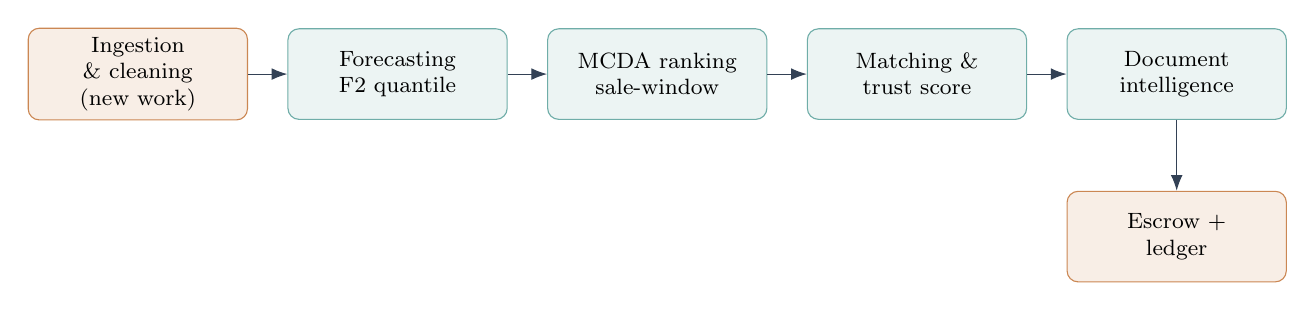
\begin{tikzpicture}[
  node distance=0.55cm and 0.5cm,
  box/.style={draw, rounded corners, fill=gxteal!8, draw=gxteal!60, align=center, text width=2.55cm, minimum height=1.15cm, font=\footnotesize},
  newbox/.style={draw, rounded corners, fill=gxamber!10, draw=gxamber!70, align=center, text width=2.55cm, minimum height=1.15cm, font=\footnotesize},
  arr/.style={-{Latex[length=2mm]}, draw=gxslate}
]
\node[newbox] (ing) {Ingestion \& cleaning\\(new work)};
\node[box, right=of ing] (fc) {Forecasting\\F2 quantile};
\node[box, right=of fc] (rk) {MCDA ranking\\sale-window};
\node[box, right=of rk] (mt) {Matching \&\\trust score};
\node[box, right=of mt] (doc) {Document\\intelligence};
\node[newbox, below=0.9cm of doc] (chain) {Escrow +\\ledger};
\draw[arr] (ing) -- (fc);
\draw[arr] (fc) -- (rk);
\draw[arr] (rk) -- (mt);
\draw[arr] (mt) -- (doc);
\draw[arr] (doc) -- (chain);
\end{tikzpicture}
\end{center}

\renewcommand{\arraystretch}{1.35}
\noindent\begin{longtable}{@{}p{2.9cm}p{0.5cm}p{9.4cm}@{}}
\toprule
\textbf{Stage} & & \textbf{What it does, and its real status} \\
\midrule
\endhead
Ingestion \& cleaning & \bld & \textbf{New work.} Daily pull from Agmarknet/AIKosh mandi feeds, normalised
into the same shape the existing trade-panel pipeline expects: commodity, market, date, min/modal/max
price, arrival quantity. Needs a canonical commodity/unit lookup table and a gap-fill policy --- see
Section 2 for exactly why. \\[0.4em]
Forecasting & \pmid & Two forecasters exist. \textbf{F1} (Dual-Head GRU) is real but its own benchmark file
shows it underperforming a plain moving average (54.49\% MAPE vs.\ 29.42\%) --- do not lead with it.
\textbf{F2} (XGBoost quantile forecaster) is the one to use: it produces a price \emph{band}, not a bare
number, which is both more honest and the right shape for a hold/sell recommendation. Needs recalibration
on real mandi data before the demo --- it was validated on trade-corridor data, not this domain. \\[0.4em]
Ranking (sale-window) & \yes & The existing MCDA destination-ranking engine (R1) --- explainable, 8 weighted
dimensions, backtested $\rho = 0.884$, precision@5 of 0.8 on a real 48{,}445-row dataset. Repurposed here to
rank \{sell now at market A, sell now at market B, hold $N$ days\} using price-trend, storage-cost,
transport-cost and glut-risk dimensions instead of tariff/logistics/demand. Reused almost unmodified. \\[0.4em]
Matching \& trust score & \pmid & Route through the real company-directory endpoint (TF-IDF + cosine +
valuation blending), \textbf{not} \texttt{counterparty\_controller.py}'s stub path, which still generates
fake data via an \texttt{hashlib.md5} seed. The trust score itself should ultimately be read from the
on-chain reputation ledger (Section 3), not just computed in the app layer, for the same reason escrow
matters --- a number nobody can quietly edit. \\[0.4em]
Document intelligence & \yes & Rule-based OCR/NER + cross-document reconciliation (not ML, and that's fine
to say plainly). Checks a grading certificate against the lot record the same way it checks an invoice
against a bill of lading today. Feeds a SHA-256 hash of the certificate into the ledger anchor. \\[0.4em]
Escrow + ledger & \pmid & Real, working code --- see Section 3 in full. \texttt{ESCROW\_ENABLED} currently
defaults off and needs to be turned on, tested, and have one access-control gap fixed before demo. \\
\bottomrule
\end{longtable}

\begin{warnbox}{The trade anomaly/risk stack is available but not core to this pipeline}
The 0.98 F1 anomaly classifier and the Isolation Forest + GRU risk ensemble exist and are GlobeX's most
rigorously validated components, but they were built for trade-corridor fraud patterns. They \emph{could}
be repurposed as an optional ``suspicious listing/price manipulation'' check on the marketplace side, but
that is a stretch addition, not part of the core 26132 pipeline --- don't let it distract from the five
stages above.
\end{warnbox}

% ================= DATASET =================
\clearpage
\section{The data behind it}

\subsection*{What's genuinely public}
\renewcommand{\arraystretch}{1.3}
\noindent\begin{longtable}{@{}p{4.3cm}p{8.5cm}@{}}
\toprule
\textbf{Source} & \textbf{What it actually gives you} \\
\midrule
\endhead
Agmarknet, via data.gov.in (OGD) & Daily state/district/market-level mandi prices (min/modal/max) and
arrival quantities. Resource ID \texttt{9ef84268-d588-465a-a308-a864a43d0070} for the main dataset, plus a
variety-wise companion resource. Free API key from a data.gov.in account; JSON or CSV. \\[0.3em]
AIKosh (IndiaAI Mission, MeitY) & The same data, repackaged specifically for AI use --- worth citing
alongside data.gov.in since it's the government's own ``curated for AI'' platform. \\[0.3em]
CEDA Agri Market Data (Ashoka Univ.) \& India Data Portal & Cleaner mirrors of the same underlying DMI
source, good for fast prototyping before wiring the live API. \\[0.3em]
AGMARK grading standards & The grade specifications themselves (moisture, size, foreign-matter thresholds
per commodity) are public --- useful as the rule set document intelligence checks against. \\
\bottomrule
\end{longtable}

\begin{codebox}
GET https://api.data.gov.in/resource/9ef84268-d588-465a-a308-a864a43d0070\\
    ?api-key=\{your\_key\}\&format=json\&offset=0\&limit=100\\
    \&filters[state]=Maharashtra\&filters[commodity]=Onion
\end{codebox}

\subsection*{What's genuinely absent --- do not claim these as sourced}
\renewcommand{\arraystretch}{1.3}
\noindent\begin{longtable}{@{}p{4.3cm}p{8.5cm}@{}}
\toprule
\textbf{Gap} & \textbf{Honest handling} \\
\midrule
\endhead
FPO / buyer directory \& credentials & No public dataset anywhere. Build a small, clearly-labelled pilot
seed set (50--150 records) and say so in the pitch: ``pilot seed data; onboarding real FPOs is the first
90-day milestone.'' \\[0.3em]
Actual graded-lot records & Standards are public, graded outcomes are not. Verify against documents, don't
claim a trained grading model. \\[0.3em]
Storage/warehouse capacity \& pricing & WDRA publishes a registered-warehouse list only --- no live capacity
or price data. Treat storage cost as an assumption input for the demo. \\[0.3em]
eNAM transaction data & eNAM's dashboard just re-displays the same Agmarknet data --- it is not an
independent source or an open API. Frame any eNAM mention as a future partnership, not a built integration. \\
\bottomrule
\end{longtable}

\begin{warnbox}{Data-quality issues to budget real time for}
Inconsistent commodity/variety naming across states, missing reporting days, non-standard units, an API
that can return an empty page before its own reported total is reached, and some older resources that
ignore the requested output format and always return CSV. None of these are modelling problems --- they are
ingestion-layer work, and they decide whether the live demo actually works.
\end{warnbox}

% ================= BLOCKCHAIN =================
\clearpage
\section{Blockchain \& escrow --- how it really works}
Verified directly from the chain-adapter repo's code, not a generic description.

\subsection*{Two payment rails, one chosen per escrow}
\textbf{RAZORPAY} --- real rupees, UPI/cards, no crypto wallet needed. \textbf{This is the rail for
farmers.} \textbf{CRYPTO} --- a real contract (\texttt{CryptoEscrow.sol}) deployed on Ethereum Sepolia
(chain ID 11155111), holding native ETH or a test ERC-20 token (\texttt{GlobexUSD.sol}, symbol
\texttt{gUSD}). GlobeX's backend owns create/release/refund/dispute on this contract; only the deposit is
signed by the payer's own wallet. Every crypto payment is re-verified straight from the chain (right
contract, right sender, right amount, right trade ID) before being marked funded --- never trusts a webhook.

\subsection*{The escrow state machine (same shape, whichever rail is used)}
\begin{center}
\small
CREATED $\to$ AWAITING\_PAYMENT $\to$ FUNDED $\to$ IN\_SHIPMENT $\to$ DELIVERED $\to$ INSPECTION $\to$
\{RELEASED \textbar\ DISPUTED\} $\to$ \{RELEASED \textbar\ REFUNDED\}
\end{center}
For 26132: offer accepted $\to$ buyer pays $\to$ lot picked up $\to$ lot delivered $\to$ grading checked
$\to$ funds released, or disputed if the grade doesn't match what was promised.

\subsection*{The permanent record book --- \texttt{TradeLedger.sol}}
Separate from the money entirely. Once a trade settles, one record is written on-chain: product, quantity,
amount, expected vs.\ actual delivery, inspection result, dispute status, settlement status, a SHA-256
fingerprint of the invoice/grading certificate, and a timestamp. The contract itself auto-computes a
running reputation score per farmer/FPO from this history --- completed, disputed, on-time, quality-passed
trade counts and a current trust score --- so the number is calculated, not typed in by anyone. This is
written \emph{regardless} of which payment rail was used --- record-keeping and money movement are
independent.

\begin{redbox}{Fix before claiming any of this is tamper-proof}
\texttt{TradeLedger.recordTrade()} is currently \texttt{public} with \textbf{no access control} --- no
\texttt{onlyOwner}, unlike \texttt{CryptoEscrow.sol} where every state-changing function is locked to the
owner. Right now, anyone with the contract address could call it directly and write a fake trade record or
inflate a trust score. This must be locked down (owner-only or signature-gated, matching the escrow
contract's pattern) before any pitch claims the trust score can't be faked --- a technical judge could
disprove that claim live on a block explorer otherwise.
\end{redbox}

\begin{uspbox}{How to pitch this to a farmer audience}
The PS never asks for blockchain by name --- it asks for payment reliability and transparent records, which
is an outcome, not a technology mandate. Lead with the outcome (``your money is held until your grain is
confirmed delivered and graded''; ``your trading history can't be faked by anyone, including us''), keep
every bit of wallet/gas/chain-ID plumbing invisible to the farmer UI, and only explain the on-chain
mechanism if a judge specifically asks how the guarantee is enforced.
\end{uspbox}

% ================= BUILD PLAN =================
\clearpage
\section{What still needs to be built --- one prioritised list}

\subsection*{Fix first --- small effort, removes real credibility risk}
\begin{enumerate}[leftmargin=1.6em]
\item Lock down \texttt{TradeLedger.recordTrade()} with an owner-only or signature-gated check.
\item Reconcile the README's 8.42\% MAPE claim against \texttt{benchmark\_comparison.csv}'s 54.49\% ---
either retrain and report honestly, or switch the headline to F2's real number and drop the GRU figure.
\item Route ``verified buyer'' matching through the real company-directory endpoint, not the
\texttt{md5}-seeded stub in \texttt{counterparty\_controller.py}.
\item Flip \texttt{ESCROW\_ENABLED} on, add version-controlled DB migrations (only one exists today), and
dry-run the full fund $\to$ release and fund $\to$ dispute $\to$ resolve paths on testnet repeatedly.
\end{enumerate}

\subsection*{Must-have for the demo to work at all}
\begin{itemize}[leftmargin=1.4em]
\item Real, cleaned Agmarknet/AIKosh ingestion for 2--3 states and a handful of commodities.
\item F2 quantile forecaster recalibrated on that real mandi data, presented as a band, not a number.
\item MCDA ranking repurposed into the sale-window recommender.
\item Matching against a labelled pilot FPO/buyer seed dataset, through the real endpoint, trust score
visible.
\item Escrow happy path (Razorpay rail) live end-to-end, with the ledger entry visible in the UI.
\item A clickable front-end flow, start to finish, no narration filling gaps.
\end{itemize}

\subsection*{Should-have --- strengthens the pitch}
\begin{itemize}[leftmargin=1.4em]
\item Dispute path demoed live, not described.
\item Document/grading verification shown against a real sample certificate.
\item Reputation/audit-trail view exposed in the UI, pulled from \texttt{TradeLedger}, not just the DB.
\item Coverage widened to 4--5 states once the core flow is solid.
\end{itemize}

\subsection*{Could-have --- genuine stretch, don't commit}
\begin{itemize}[leftmargin=1.4em]
\item Image-based grade classifier, only if a labelled photo dataset can be assembled in time.
\item Vernacular-language or WhatsApp-bot front end.
\item Marketplace-side reuse of the anomaly/risk stack for suspicious-listing detection.
\end{itemize}

\subsection*{Won't-have --- say so upfront, don't apologise}
\begin{itemize}[leftmargin=1.4em]
\item Live eNAM transaction data or GSTN/bank payment-rail integration.
\item Nationwide commodity coverage at launch.
\item A trained (rather than rules-based) grading model, unless the stretch goal above is actually reached.
\end{itemize}

\section*{Bottom line}
The AI pipeline is four-fifths already built --- ingestion is the one genuinely new component, and it's data
engineering, not modelling. The core dataset this idea needs is solidly public and API-accessible today.
The blockchain/escrow layer is real, working code, not a slide, with one access-control bug to fix and a
default-off flag to switch on. Everything the PS asks for maps to something that exists; what's left is
closing four small, well-defined gaps and doing the unglamorous ingestion work --- not inventing new
capability.

\end{document}
